\documentclass[../ClassicThesis.tex]{subfiles}
\begin{document}

%************************************************
\chapter{Assembly}\label{ch:assembly}
%************************************************
\section{somebody will have to do the following sections shortly}

Assembling the laser cut models is not trivial. Since multiple plates may be very similar to each other, it is not always clear which have to be put together. Thus, we decided to add assembly instructions, which allow the user to assemble the model hassle-free. Section \ref{sub:assemlyplates} describes how these instructions are added to plates which were found either inherently or by extruding. The assembly instructions for stacked plates are discussed in Section \ref{sub:assemblystacked}.

\section{What we currently have (not good solution)}

This section describes the currently used methods for adding assembly instructions. While these do simplify assembly, they are not optimal. Ideas for improvement are discussed in Section \ref{sec:assemblyimprovements}.

\subsection{Plate method}\label{sub:assemblyplates}

%just write numbers on lines -> equal numbers belong together

Plates created by the \emph{Plate method} \fabmethod are connected by finger joints. In order to show which plates have to be put together, the corresponding edges are annotated accordingly.

\begin{figure}
    \centering
    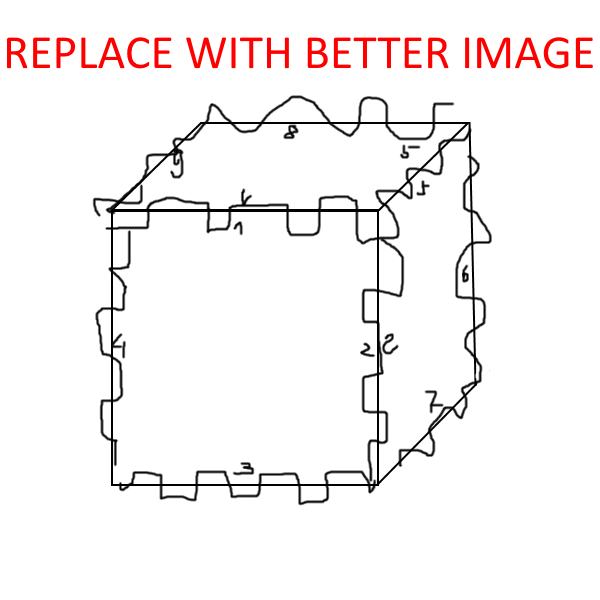
\includegraphics[width=0.5\columnwidth]{Images/assembly_plates.png}
    \caption{Assembly instructions for plates connected by finger joints.}
    \label{fig:assemblyplates}
\end{figure}

\subsection{Stacked-method}\label{sub:assemblystacked}

\begin{figure}
    \centering
    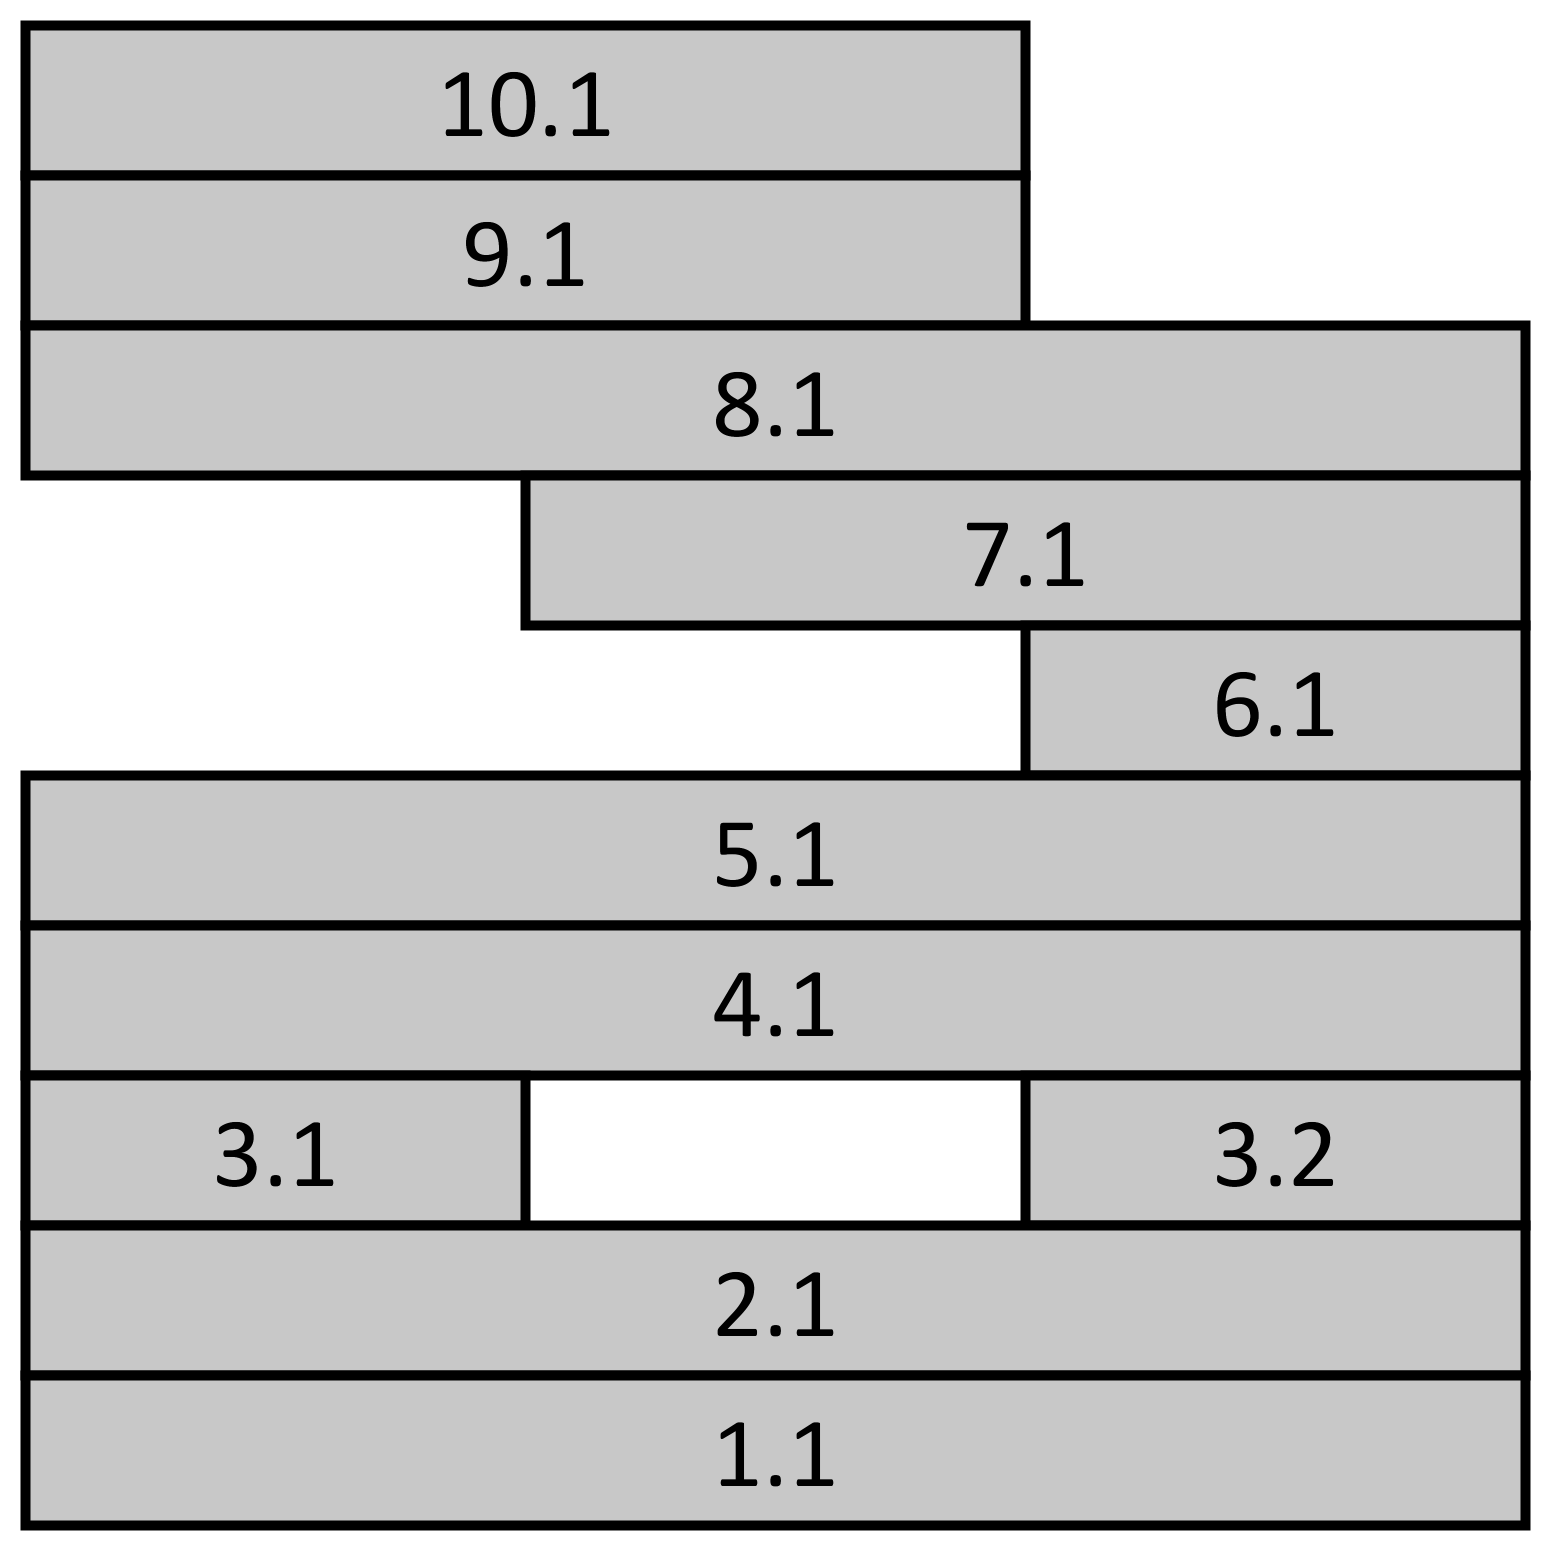
\includegraphics[width=0.5\columnwidth]{Images/assembly_stacked.png}
    \caption{Assembly intructions for stacked plates.}
    \label{fig:assemblystacked}
\end{figure}

%number plates



\section{What might be better, but is not implemented}\label{sec:assemblyimprovements}
\subsection{Idea 1: images showing if plate is horizontal or vertical etc}
\subsection{Idea 2: large number in the middle of the plate}

\end{document}